Ocurre cuando una onda se encuentra con un obstáculo o abertura y se desvía, propagándose en diferentes direcciones. Puede producirse de distinas formas dependiendo del tamaño del obstáculo y la longitud de onda de la onda. Puede ocurrir alrededor o a través de un obstáculo o abertura. En este proceso se crean zonas en donde las onda no llegan o se cancelan mediante interfernecia \textbf{destructiva}.

\begin{figure}[H]
  \centering
  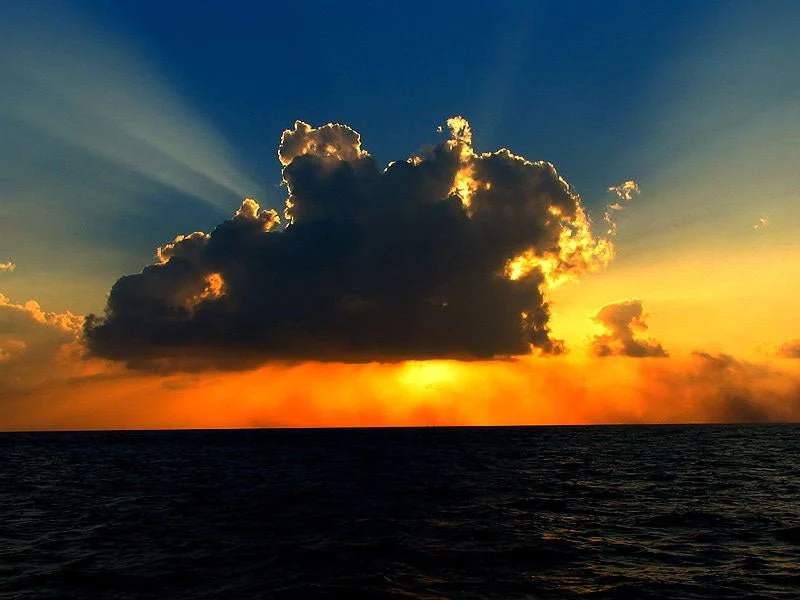
\includegraphics[scale=0.3]{imagenes/difraccion_nube.png}
  \caption{Difracción en las nubes\cite{rnbsymdfr}}
\end{figure}

Una forma simple de ver la difracción de ondas es colocar los dedos de una mano en frente de una fuente de luz y cerrarlos lentamente observando la luz pasar a través de ellos. A medida que los dedos se acercan unos a otros la luz forma patrones de lineas entre los dedos. Otra situación de esto es la luz difractada por las nubes. Esas lineas son patrones de difracción\cite{sncdfrlight}.
